\begin{titlepage}
\newcommand{\HRule}{\rule{\linewidth}{0.5mm}} 							% horizontal line and its thickness
\center 
%\flushright
% University
\textsc{\huge Gábor Dénes Főiskola}\\[1cm]

% Document info
\textsc{\LARGE Mérnökinformatikus alapképzés}\\[0.2cm]
\HRule \\[0.8cm]
{\huge \bfseries \@title}\\[0.7cm]								% Assignment
\HRule \\[2cm]

% Author
{\LARGE \bfseries
\@author}\\[1.5cm]
%Supervisor
{\Large Konzulens:\\[0.5cm]
Dr. Nagy Elemér Károly}\vspace{2cm}

{\LARGE Szoftverfejlesztés szakirány}\\[0.5cm]					    % Course Code


\includegraphics[height=0.2\textwidth]{gdf_logo.png}

\vfill
{\Large \monthyeardate{\@date}}
\end{titlepage}

\thispagestyle{empty}
\cleardoublepage

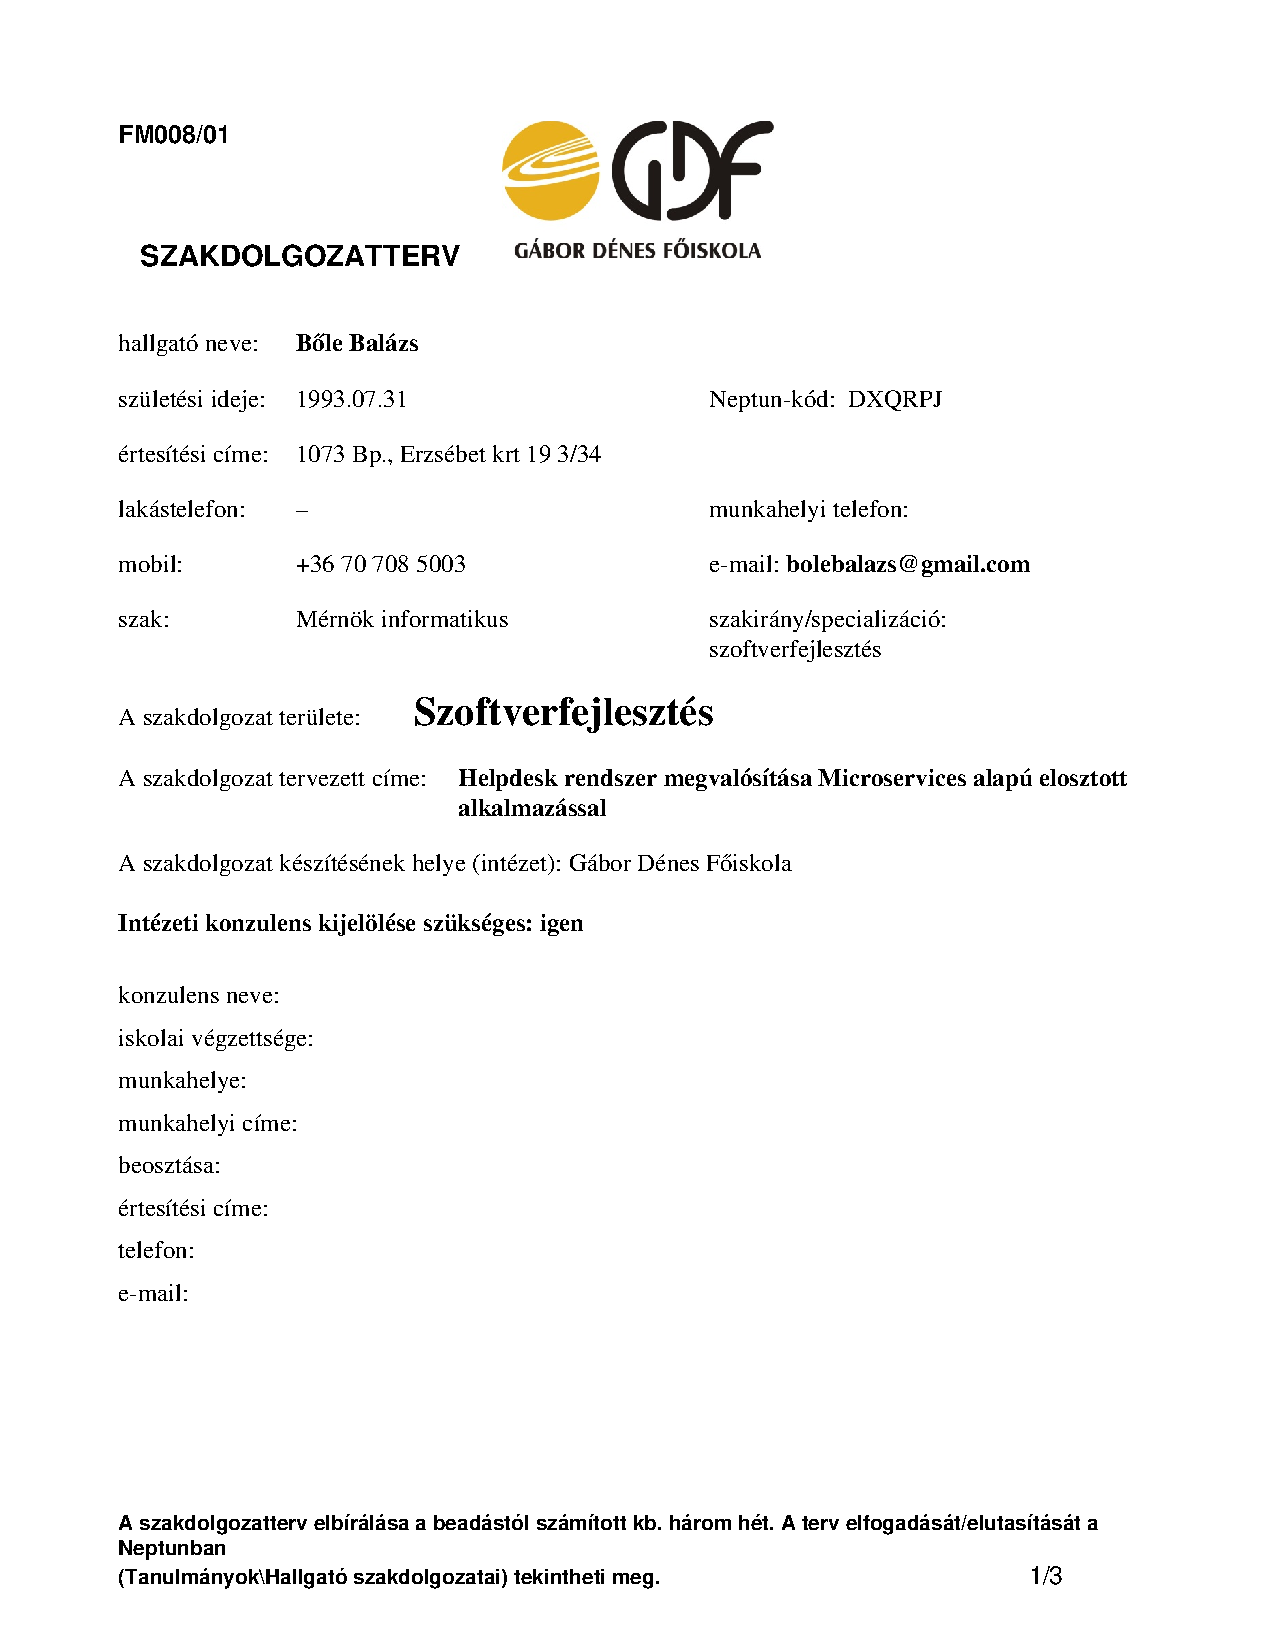
\includepdf[pages=-]{FM008_01_Szakdolgozatterv-DXQRPJ.pdf}
\cleardoublepage

\includepdf[pages=-]{eredetiseg-nyilatkozat.pdf}

\thispagestyle{empty}
\cleardoublepage

\thispagestyle{empty}
\begin{center}
	{\Large \bfseries \@title}
	
	\bigskip
	\bigskip
	
	készítette
	
	\bigskip
	\bigskip
	
	{\large \bfseries \@author}
	
	\bigskip
	
	\vfill
	
	\begin{tabular}{ll}
		Neptun kód: & DXQRPJ \\
		Elérhetőség: & \href{mailto:bolebalazs@gmail.com}{bolebalazs@gmail.com}\\
		
		\bigskip\\
		
		Konzulens: & Dr.\ Nagy\ Elemér\ Károly
		

	\end{tabular}

	\bigskip
	\bigskip

\mbox{A dolgozat elektronikus változata elérhető a \url{https://github.com/balazsBole/} címen.}	
	

	
	\bigskip
	
	
\includegraphics[width=0.2\textwidth]{gdf_logo.png}

	
\end{center}
Budapest, \monthyeardate{\@date}.
